% Created 2020-09-13 Sun 10:09
% Intended LaTeX compiler: pdflatex
\documentclass[11pt]{article}
\usepackage[utf8]{inputenc}
\usepackage[T1]{fontenc}
\usepackage{graphicx}
\usepackage{grffile}
\usepackage{longtable}
\usepackage{wrapfig}
\usepackage{rotating}
\usepackage[normalem]{ulem}
\usepackage{amsmath}
\usepackage{textcomp}
\usepackage{amssymb}
\usepackage{capt-of}
\usepackage{hyperref}
\author{srolisp}
\date{\textit{<2020-09-12 Sat 18:00>}}
\title{SVM, k-means\\\medskip
\large 4 weeks by kdh}
\hypersetup{
 pdfauthor={srolisp},
 pdftitle={SVM, k-means},
 pdfkeywords={},
 pdfsubject={},
 pdfcreator={Emacs 28.0.50 (Org mode 9.3)}, 
 pdflang={English}}
\begin{document}

\maketitle
\tableofcontents


\section{알고리즘보다는 파이썬에 익숙해지는데 시간을 들이고, 전체적인 flow를 익히자.}
\label{sec:orgdba01d1}

\section{SVM(Support Vector Machine)}
\label{sec:org0063863}
광장히 많이 쓰여지고 있는 알고리즘이다. 지도학습이다. 결정된 점들의 최대 마진을 가지는 선을 찾는 알고리즘을 적용한 것이다. 

\subsection{SVM 실습}
\label{sec:org19cc79c}
\begin{verbatim}
import numpy as np
import matplotlib.pyplot as plt
from sklearn import svm
from sklearn.datasets import make_blobs
\end{verbatim}

랜덤스테이트 값이 정해지면 포인트도 매번 동일한가. 값이 값네..
make\textsubscript{blobs}: 학습용 데이터셋을 만들어주는 함수라고 하네. 
\begin{verbatim}
# we create 40 separable points
X, y = make_blobs(n_samples=40, centers=2, random_state=6)
X
\end{verbatim}

\begin{verbatim}
array([[  6.37734541, -10.61510727],
[  6.50072722,  -3.82403586],
[  4.29225906,  -8.99220442],
[  7.39169472,  -3.1266933 ],
[  7.64306311, -10.02356892],
[  8.68185687,  -4.53683537],
[  5.37042238,  -2.44715237],
[  9.24223825,  -3.88003098],
[  5.73005848,  -4.19481136],
[  7.9683312 ,  -3.23125265],
[  7.37578372,  -8.7241701 ],
[  6.95292352,  -8.22624269],
[  8.21201164,  -1.54781358],
[  6.85086785,  -9.92422452],
[  5.64443032,  -8.21045789],
[ 10.48848359,  -2.75858164],
[  7.27059007,  -4.84225716],
[  6.29784608, -10.53468031],
[  9.42169269,  -2.6476988 ],
[  8.98426675,  -4.87449712],
[  6.6008728 ,  -8.07144707],
[  5.95313618,  -6.82945967],
[  6.87151089, -10.18071547],
[  6.26221548,  -8.43925752],
[  7.97164446,  -3.38236058],
[  7.67619643,  -2.82620437],
[  7.92736799,  -9.7615272 ],
[  5.86311158, -10.19958738],
[  8.07502382,  -4.25949569],
[  6.78335342,  -8.09238614],
[  7.89359985,  -7.41655113],
[  6.04907774,  -8.76969991],
[  6.77811308,  -9.80940478],
[  8.71445065,  -2.41730491],
[  8.49142837,  -2.54974889],
[  9.49649411,  -3.7902975 ],
[  7.52132141,  -2.12266605],
[  6.3883927 ,  -9.25691447],
[  7.93333064,  -3.51553205],
[  6.86866543, -10.02289012]])
\end{verbatim}

\begin{verbatim}
# fit the model, don't regularize for illustration purposes
clf = svm.SVC(kernel='linear', C=1000)
clf.fit(X, y)
\end{verbatim}

\begin{verbatim}
SVC(C=1000, kernel='linear')
\end{verbatim}

\begin{verbatim}
plt.scatter(X[:, 0], X[:, 1], c=y, s=30, cmap=plt.cm.Paired)
\end{verbatim}

\begin{verbatim}
<matplotlib.collections.PathCollection at 0x7ffcc4b57f98>
\end{verbatim}

\begin{center}
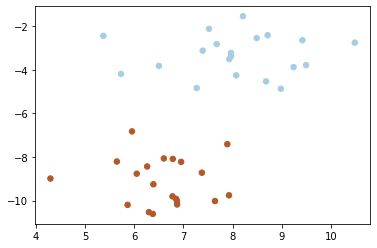
\includegraphics[width=.9\linewidth]{./obipy-resources/dPNazO.png}
\end{center}

좌표 x,y 수정작업
\begin{verbatim}
# plot the decision function
ax = plt.gca()
\end{verbatim}

\begin{center}
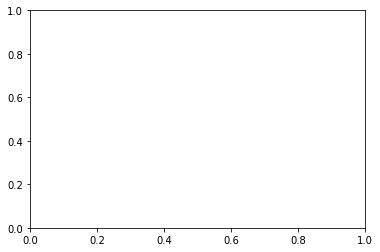
\includegraphics[width=.9\linewidth]{./obipy-resources/zNktqY.png}
\end{center}

\begin{verbatim}
xlim = ax.get_xlim()
ylim = ax.get_ylim()
xlim
\end{verbatim}

\begin{verbatim}
(0.0, 1.0)
\end{verbatim}
분리해서 실행하니 contour 에러가 떠서 결과물을 보려면 소스코드를 분리하지 말고 실행하자. 왜일까?
\begin{verbatim}
# create grid to evaluate model
xx = np.linspace(xlim[0], xlim[1], 30)
yy = np.linspace(ylim[0], ylim[1], 30)
YY, XX = np.meshgrid(yy, xx)
xy = np.vstack([XX.ravel(), YY.ravel()]).T
Z = clf.decision_function(xy).reshape(XX.shape)

# plot decision boundary and margins
ax.contour(XX, YY, Z, colors='k', levels=[-1, 0, 1], alpha=0.5, linestyles=['--', '-', '--'])
# plot support vectors
ax.scatter(clf.support_vectors_[:, 0], clf.support_vectors_[:, 1], s=100, linewidth=1, facecolor='none', edgecolors='k')

plt.show()

\end{verbatim}

\section{k-means(k-평균 알고리즘)}
\label{sec:orgbfa4e22}
주어진 데이터를 k개의 클러스터로 묶는 알고리즘이고 비지도 학습이다. 클러스티링용 알고리즘. 클래시파잉(A다 B다)은 아니다. 데이터를 군집화 하는 용도로 쓰이는 알고리즘이다.

\subsection{실습}
\label{sec:org4687527}
\begin{verbatim}
import numpy as np
import matplotlib.pyplot as plt
from sklearn.cluster import KMeans
from sklearn.metrics import pairwise_distances_argmin
from sklearn.datasets import load_sample_image
from sklearn.utils import shuffle
from time import time

n_colors = 64

# Load the Summer Palace photo
china = load_sample_image("china.jpg")
china
\end{verbatim}

\begin{verbatim}
array([[[174, 201, 231],
[174, 201, 231],
[174, 201, 231],
...,
[250, 251, 255],
[250, 251, 255],
[250, 251, 255]],

[[172, 199, 229],
[173, 200, 230],
[173, 200, 230],
...,
[251, 252, 255],
[251, 252, 255],
[251, 252, 255]],

[[174, 201, 231],
[174, 201, 231],
[174, 201, 231],
...,
[252, 253, 255],
[252, 253, 255],
[252, 253, 255]],

...,

[[ 88,  80,   7],
[147, 138,  69],
[122, 116,  38],
...,
[ 39,  42,  33],
[  8,  14,   2],
[  6,  12,   0]],

[[122, 112,  41],
[129, 120,  53],
[118, 112,  36],
...,
[  9,  12,   3],
[  9,  15,   3],
[ 16,  24,   9]],

[[116, 103,  35],
[104,  93,  31],
[108, 102,  28],
...,
[ 43,  49,  39],
[ 13,  21,   6],
[ 15,  24,   7]]], dtype=uint8)
\end{verbatim}

\begin{verbatim}
# Convert to floats instead of the default 8 bits integer coding. Dividing by
# 255 is important so that plt.imshow behaves works well on float data (need to
# be in the range [0-1])
china = np.array(china, dtype=np.float64) / 255
china
\end{verbatim}

\begin{verbatim}
array([[[0.68235294, 0.78823529, 0.90588235],
[0.68235294, 0.78823529, 0.90588235],
[0.68235294, 0.78823529, 0.90588235],
...,
[0.98039216, 0.98431373, 1.        ],
[0.98039216, 0.98431373, 1.        ],
[0.98039216, 0.98431373, 1.        ]],

[[0.6745098 , 0.78039216, 0.89803922],
[0.67843137, 0.78431373, 0.90196078],
[0.67843137, 0.78431373, 0.90196078],
...,
[0.98431373, 0.98823529, 1.        ],
[0.98431373, 0.98823529, 1.        ],
[0.98431373, 0.98823529, 1.        ]],

[[0.68235294, 0.78823529, 0.90588235],
[0.68235294, 0.78823529, 0.90588235],
[0.68235294, 0.78823529, 0.90588235],
...,
[0.98823529, 0.99215686, 1.        ],
[0.98823529, 0.99215686, 1.        ],
[0.98823529, 0.99215686, 1.        ]],

...,

[[0.34509804, 0.31372549, 0.02745098],
[0.57647059, 0.54117647, 0.27058824],
[0.47843137, 0.45490196, 0.14901961],
...,
[0.15294118, 0.16470588, 0.12941176],
[0.03137255, 0.05490196, 0.00784314],
[0.02352941, 0.04705882, 0.        ]],

[[0.47843137, 0.43921569, 0.16078431],
[0.50588235, 0.47058824, 0.20784314],
[0.4627451 , 0.43921569, 0.14117647],
...,
[0.03529412, 0.04705882, 0.01176471],
[0.03529412, 0.05882353, 0.01176471],
[0.0627451 , 0.09411765, 0.03529412]],

[[0.45490196, 0.40392157, 0.1372549 ],
[0.40784314, 0.36470588, 0.12156863],
[0.42352941, 0.4       , 0.10980392],
...,
[0.16862745, 0.19215686, 0.15294118],
[0.05098039, 0.08235294, 0.02352941],
[0.05882353, 0.09411765, 0.02745098]]])
\end{verbatim}

\begin{verbatim}
  # Load Image and transform to a 2D numpy array.
  w, h, d = original_shape = tuple(china.shape)
w
\end{verbatim}

\begin{verbatim}
427
\end{verbatim}

\begin{verbatim}
assert d == 3
image_array = np.reshape(china, (w * h, d))
image_array
\end{verbatim}

\begin{verbatim}
array([[0.68235294, 0.78823529, 0.90588235],
[0.68235294, 0.78823529, 0.90588235],
[0.68235294, 0.78823529, 0.90588235],
...,
[0.16862745, 0.19215686, 0.15294118],
[0.05098039, 0.08235294, 0.02352941],
[0.05882353, 0.09411765, 0.02745098]])
\end{verbatim}

\begin{verbatim}
print("Fitting model on a small sub-sample of the data")
t0 = time()
image_array_sample = shuffle(image_array, random_state=0)[:1000]
image_array_sample
\end{verbatim}

\begin{verbatim}
array([[0.92156863, 0.9254902 , 0.94509804],
[0.37647059, 0.37647059, 0.14117647],
[0.48235294, 0.42745098, 0.41568627],
...,
[0.96862745, 0.96862745, 0.97647059],
[0.9372549 , 0.96470588, 1.        ],
[0.11372549, 0.12156863, 0.07843137]])
\end{verbatim}

\begin{verbatim}
kmeans = KMeans(n_clusters=n_colors, random_state=0).fit(image_array_sample)
kmeans
\end{verbatim}

\begin{verbatim}
KMeans(n_clusters=64, random_state=0)
\end{verbatim}

\begin{verbatim}
print("done in %0.3fs." % (time() - t0))

codebook_random = shuffle(image_array, random_state=0)[:n_colors]
codebook_random
\end{verbatim}

\begin{verbatim}
array([[0.92156863, 0.9254902 , 0.94509804],
[0.37647059, 0.37647059, 0.14117647],
[0.48235294, 0.42745098, 0.41568627],
[0.81960784, 0.81568627, 0.84705882],
[0.98823529, 0.98823529, 0.98823529],
[0.41568627, 0.16470588, 0.16862745],
[0.94901961, 0.94901961, 0.95686275],
[0.87843137, 0.92941176, 0.99215686],
[0.24313725, 0.32156863, 0.17647059],
[0.80784314, 0.88627451, 0.98039216],
[0.07843137, 0.12941176, 0.01960784],
[0.84705882, 0.91372549, 0.97647059],
[0.75686275, 0.82745098, 0.91372549],
[0.04313725, 0.04313725, 0.04313725],
[0.38823529, 0.36470588, 0.23137255],
[0.1254902 , 0.05490196, 0.05490196],
[0.85490196, 0.92156863, 1.        ],
[0.61568627, 0.58823529, 0.42352941],
[0.80784314, 0.89411765, 0.98823529],
[0.70196078, 0.75686275, 0.75686275],
[0.86666667, 0.92941176, 0.98823529],
[0.76078431, 0.81568627, 0.85882353],
[0.03921569, 0.03921569, 0.03921569],
[0.8       , 0.87843137, 0.97647059],
[0.17647059, 0.25490196, 0.29019608],
[0.94117647, 0.95294118, 0.98039216],
[0.0745098 , 0.05882353, 0.05490196],
[0.54117647, 0.52156863, 0.27058824],
[0.74117647, 0.78431373, 0.76862745],
[0.32156863, 0.14117647, 0.14901961],
[0.89411765, 0.94901961, 1.        ],
[0.02352941, 0.        , 0.00784314],
[0.02352941, 0.03529412, 0.00784314],
[0.41568627, 0.43529412, 0.17254902],
[0.06666667, 0.03921569, 0.01568627],
[0.89411765, 0.90980392, 0.92156863],
[0.04313725, 0.04705882, 0.02352941],
[0.81568627, 0.89803922, 0.98039216],
[0.90588235, 0.90588235, 0.91372549],
[0.16862745, 0.08235294, 0.09019608],
[0.9372549 , 0.96470588, 0.98823529],
[0.38431373, 0.25882353, 0.16862745],
[0.9254902 , 0.94117647, 0.97647059],
[0.23921569, 0.3254902 , 0.31764706],
[0.59215686, 0.42352941, 0.34901961],
[0.77254902, 0.80784314, 0.8745098 ],
[0.89803922, 0.95294118, 1.        ],
[0.71764706, 0.78823529, 0.83529412],
[0.82745098, 0.90588235, 1.        ],
[0.96470588, 0.96078431, 0.98431373],
[0.87058824, 0.89803922, 0.9372549 ],
[0.09411765, 0.09803922, 0.06666667],
[0.21568627, 0.16078431, 0.10980392],
[0.25490196, 0.16470588, 0.13333333],
[0.56862745, 0.68627451, 0.69411765],
[0.72941176, 0.82352941, 0.9254902 ],
[0.81568627, 0.80784314, 0.85098039],
[0.77647059, 0.82352941, 0.81568627],
[0.32156863, 0.50588235, 0.48235294],
[0.2627451 , 0.25490196, 0.10196078],
[0.04313725, 0.0745098 , 0.02352941],
[0.90588235, 0.94509804, 0.98431373],
[0.40784314, 0.48235294, 0.12941176],
[0.81568627, 0.86666667, 0.8       ]])
\end{verbatim}

\begin{verbatim}
print("Predicting color indices on the full image (random)")
t0 = time()
labels_random = pairwise_distances_argmin(codebook_random, image_array, axis=0)
labels_random
\end{verbatim}

\begin{verbatim}
array([55, 55, 55, ..., 52, 60, 60])
\end{verbatim}

\begin{verbatim}
print("done in %0.3fs." % (time() - t0))

def recreate_image(codebook, labels, w, h):
  """Recreate the (compressed) image from the code book & labels"""
  d = codebook.shape[1]
  image = np.zeros((w, h, d))
  label_idx = 0
  for i in range(w):
    for j in range(h):
      image[i][j] = codebook[labels[label_idx]]
      label_idx += 1
  return image
# Display all results, alongside original image
plt.figure(1)
plt.clf()
plt.axis('off')
plt.title('Original image (96,615 colors)')
plt.imshow(china)

plt.figure(2)
plt.clf()
plt.axis('off')
plt.title('Quantized image (64 colors, K-Means)')
plt.imshow(recreate_image(kmeans.cluster_centers_, labels_random, w, h))

plt.figure(3)
plt.clf()
plt.axis('off')
plt.title('Quantized image (64 colors, Random)')
plt.imshow(recreate_image(codebook_random, labels_random, w, h))

plt.show()
\end{verbatim}

\begin{center}
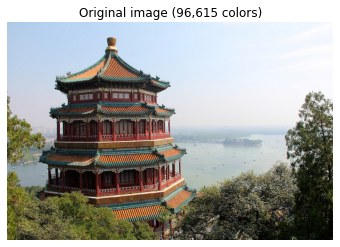
\includegraphics[width=.9\linewidth]{./obipy-resources/x2RJsY.png}
\end{center}

\subsection{make\textsubscript{blobs}}
\label{sec:org069d211}
모든 방향으로 같은 성질을 가지는 정규분포를 이용해 가상 데이터 생성해주는 함수이다. 클러스트링 용 가상데이터를 생성하는데 사용.
n\textsubscript{samples}: 표본 데이터 수
n\textsubscript{features}: 독립 변수 수
centers: 클러스터 수
cluster\textsubscript{std}: 클러스터 표준 편차
\ldots{}
\begin{verbatim}
from matplotlib import pyplot as plt
from sklearn.datasets import make_blobs

plt.title('3 clusters')
X, y = make_blobs(n_samples=300, n_features=2, centers=3, random_state=3)
plt.scatter(X[:, 0], X[:, 1], marker='o', c=y, s=30, edgecolor="k", linewidth=2)
plt.xlabel("X1")
plt.ylabel("X2")
plt.show()
\end{verbatim}

\begin{center}
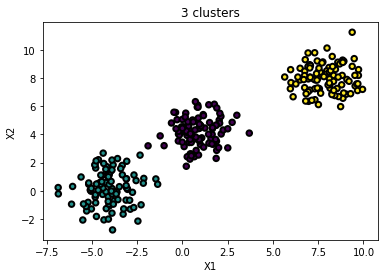
\includegraphics[width=.9\linewidth]{./obipy-resources/s4T8IX.png}
\end{center}

\section{Apriori(연관규칙)}
\label{sec:orgefa1f0d}
비지도 학습. 연관규칙중 가장 먼저 개발. 높은 빈도를 가지는 조합을 찾아내는 목적. 

장바구니 분석이라고도 함.

세가지를 주의깊게 보자.
\begin{itemize}
\item 지지도(Support): 아이템 A,B 모두 구매하는 비율
조건이 일어날 확률(달걀을 살 확률, 라면을 살 확률, ..)
\item 신뢰도(Confidence): 아이템(A)을 구매한 경우, 아이템(B)를 얼마나 구매할 것인지(라면을 샀을 때 달결을 살 확률..)
\item 향상도(Lift): B만 구매할 때보다, A를 구매한 사람이 B를 구매할 확률이 얼마나 더 높은지(동시에 얼마나 발생하는지를 비율로) <-- TODO: 다시 정리해보자
\end{itemize}

ratsgo.github.io에 자세히 설명해둔게 있다.

sparce matrix가 주로 된다(희소행렬). 희소행렬이 ai에선 많이 사용된다. 그래서 희소행렬관련 함수가 잘 만들어져있다.


\subsection{Apriori 알고리즘}
\label{sec:org9def65d}
빈발하지 않는 집합을 제거해간다. 최소지지도를 만족하지 못하는 탐색해볼 필요가 없다.


\section{머신러닝 치트 시트}
\label{sec:orge9fe329}

\subsection{\url{https://docs.microsoft.com/en-us/azure/machine-learning/algorithm-cheat-sheet}}
\label{sec:org7df45e7}

\subsection{\url{https://blogs.sas.com/content/subconsciousmusings/2017/04/12/machine-learning-algorithm-use/}}
\label{sec:org9a6665a}

\subsection{\url{http://machinelearningmastery.com/a-tour-of-machine-learning-algorithms/}}
\label{sec:orgd1a1a07}

\subsection{\ldots{}}
\label{sec:org436a960}

\section{Data Science Roadmap 2020}
\label{sec:orgfa9b18b}

\subsection{\ldots{}}
\label{sec:orgbf99e36}

\subsection{Data science roadmap}
\label{sec:org071830e}

\subsubsection{\url{https://medium.com/@ArtisOne/data-science-roadmap-2020-b256fb948404}}
\label{sec:orgf45a5c8}
\end{document}
